\section{РЕЗУЛЬТАТЫ ЖАНРОВОЙ КЛАССИФИКАЦИИ}
\label{sec:genre_classification}


Для проверки значимости выделенных образов было принято решения проверить их на задаче жанровой классификации. 

В качестве исходной выборки был использован репозиторий GZTAG. Набор данных состоит из 1000 звуковых дорожек каждые по 30 секунд. Он содержит 10 жанров, каждый из которых представлен 100 треками. Все треки - это все 220-мегагерцовые Mono 16-битные аудиофайлы в формате .wav.


Для решения задачи классификации была использована библиотека scikit-learn -- бесплатная библиотека для машинного обучения с открытым исходным кодом для языка программирования Python. Все методы классификации использованы с параметрами по умолчанию. 

\subsection{AdaBoost с деревьями принятия решений}


\begin{figure}[h]
\centering
  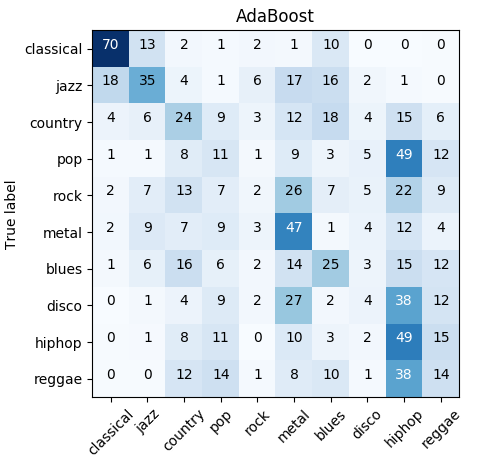
\includegraphics{AdaBoost.png}
  \caption{Матрица ошибок полученная с помощь метода классификации AdaBoost SAMME, где используется <<комитет>>  деревьев принятия решений.}
  \label{fig:results:adaboost}
\end{figure}


\begin{figure}[h]
\centering
  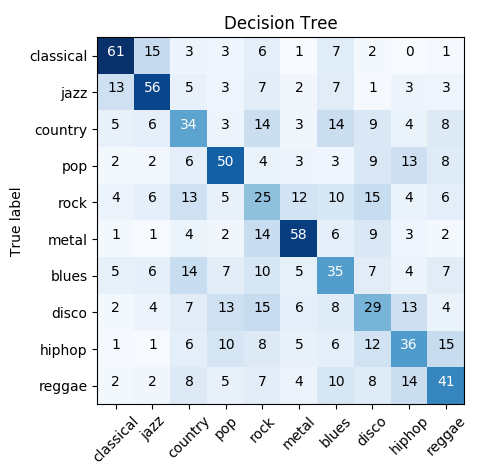
\includegraphics{DecisionTree.png}
  \caption{Матрица ошибок полученная с помощь дерева принятия решения}
  \label{fig:results:DecisionTree}
\end{figure}


\begin{figure}[h]
\centering
  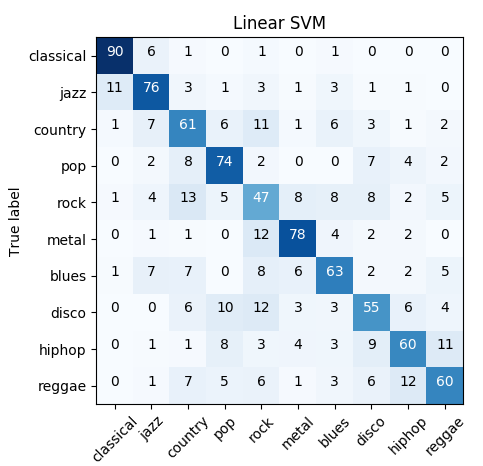
\includegraphics{LinearSVM.png}
  \caption{Матрица ошибок полученная с помощь метода опорных векторов}
  \label{fig:results:LinearSVM}
\end{figure}


\begin{figure}[h]
\centering
  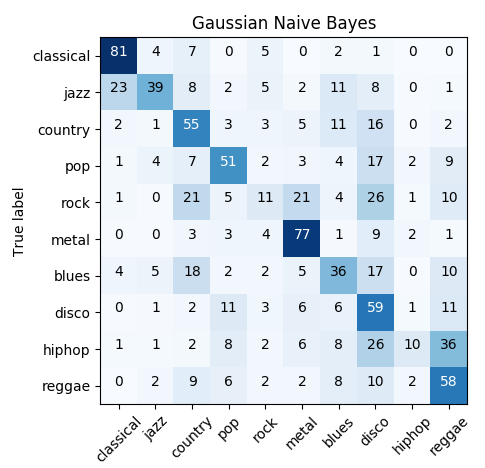
\includegraphics{NaiveBayes.png}
  \caption{Матрица ошибок полученная с помощь наивного баесовского классификатора}
  \label{fig:results:NaiveBayes}
\end{figure}

\begin{figure}[h]
\centering
  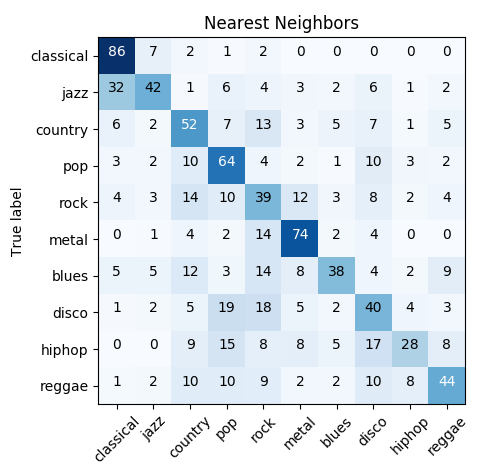
\includegraphics{NearestNeighbors.png}
  \caption{Матрица ошибок полученная с помощь метода k ближайших соседей}
  \label{fig:results:NearestNeighbors}
\end{figure}

\begin{figure}[h]
\centering
  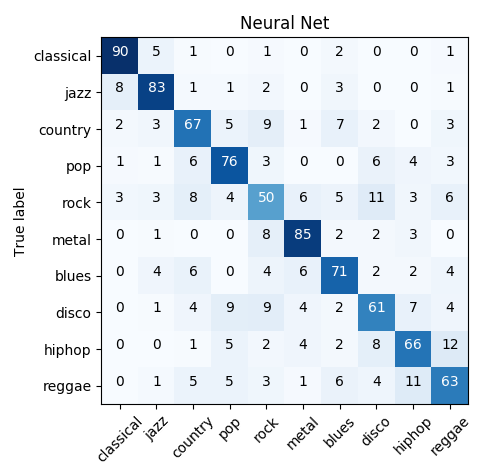
\includegraphics{NeuralNet.png}
  \caption{Матрица ошибок полученная с помощь многослойного перцептрона}
  \label{fig:results:NeuralNet}
\end{figure}


\begin{figure}[h]
\centering
  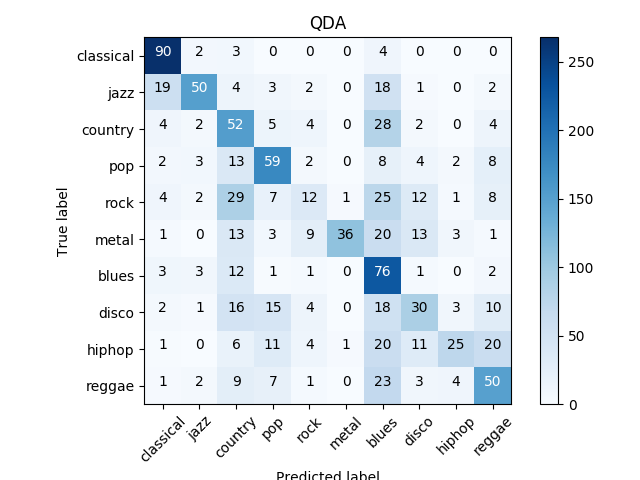
\includegraphics{QDA.png}
  \caption{Матрица ошибок полученная с помощь QDA}
  \label{fig:results:QDA}
\end{figure}


\begin{figure}[h]
\centering
  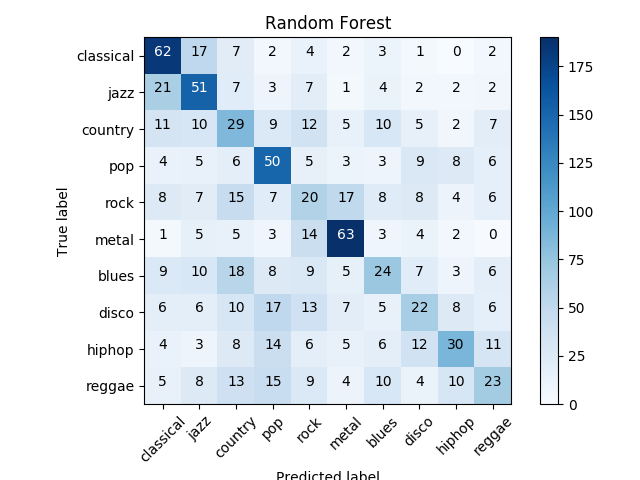
\includegraphics{RandomForest.png}
  \caption{Матрица ошибок полученная с случайного леса}
  \label{fig:results:RandomForest}
\end{figure}


В результате даже самые элементарные алгоритмы классификации показали свою эффективность, что показывает, что выделенные информационные образы значимы и могут быть использованны в системах рекомендации музыки. 


\section{РЕЗУЛЬТАТЫ ВИЗУАЛИЗАЦИИ}
\label{sec:genre_classification}





